\documentclass[tikz]{standalone}
\usepackage{tikz}
\usepackage{amsmath}
\usetikzlibrary{calc}
\usetikzlibrary{positioning}
\usetikzlibrary{fit}
\usetikzlibrary{backgrounds}
\usetikzlibrary{shapes.geometric}

\definecolor{lightGreen}{HTML}{d5e8d4}
\definecolor{lightYellow}{HTML}{fff2cc}
\definecolor{lightGray}{HTML}{f5f5f5}
\definecolor{lightRed}{HTML}{ff9999}
\definecolor{lightBlue}{HTML}{d5e5fc}
\definecolor{lightCyan}{HTML}{a7dfe3}
\pgfdeclarelayer{main_bg}
\pgfdeclarelayer{back_bg}
\pgfsetlayers{main_bg,main}


\newcommand{\mem}[2]{
    \begin{scope}
        \node (#1) [draw, rectangle, text width=\cellWidth, minimum width=\cellWidth*8, minimum height=\cellHeight, #2] {};
        \node (#1_cell_0) [draw, rectangle, text width=\cellWidth, minimum width=\cellWidth, minimum height=\cellHeight, right=0.0pt of #1.west, anchor=west] {};
        \foreach \x in {1,...,7} {
            \pgfmathtruncatemacro{\prev}{\x-1}
            \node (#1_cell_\x) [draw, rectangle, text width=\cellWidth, minimum width=\cellWidth, minimum height=\cellHeight, right=-\the\pgflinewidth of #1_cell_\prev] {};
        }
    \end{scope}
}

\begin{document}
    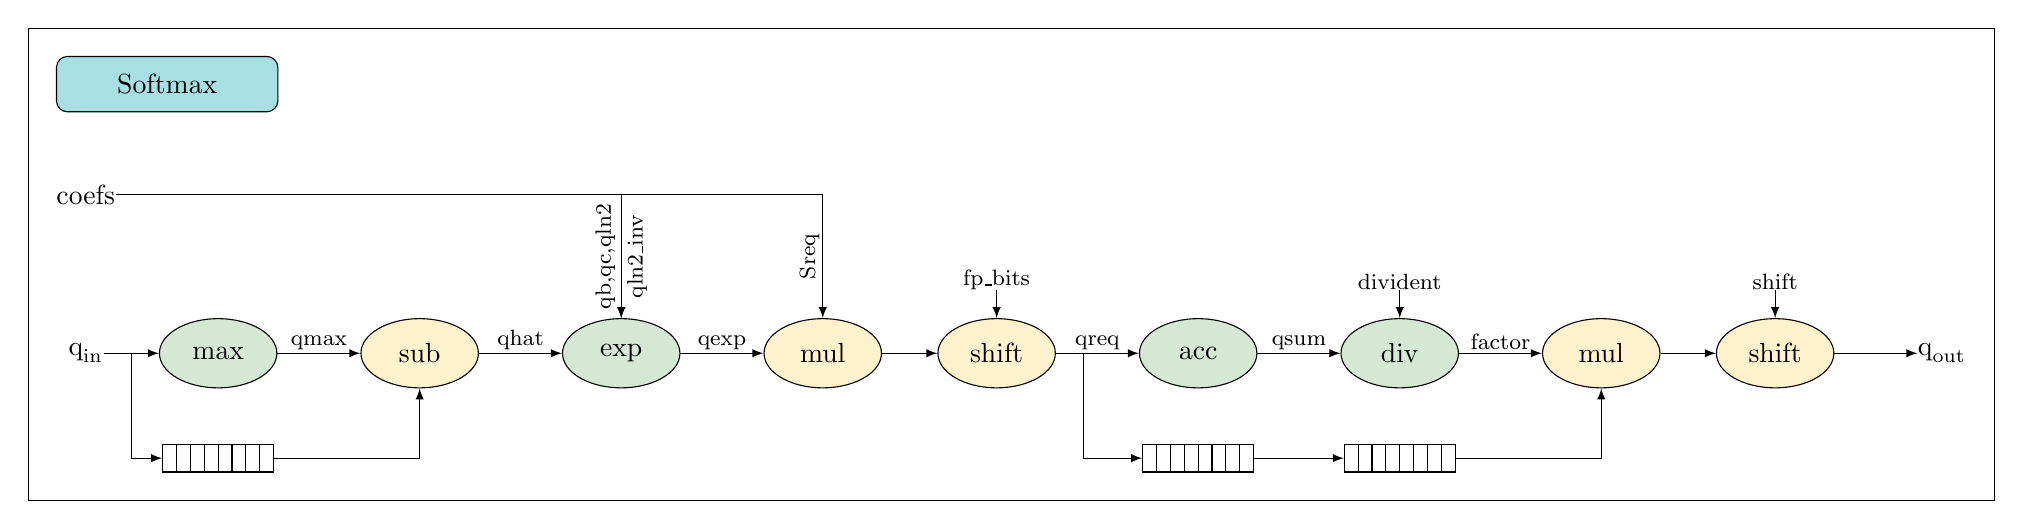
\begin{tikzpicture}[inner sep=0.0 pt, align=center]
    \pgfmathsetmacro{\rectWidth}{40}
    \pgfmathsetmacro{\rectHeight}{40}
    \pgfmathsetmacro{\ellWidth}{30}
    \pgfmathsetmacro{\ellHeight}{25}
    \pgfmathsetmacro{\cellWidth}{5}
    \pgfmathsetmacro{\cellHeight}{10}

    \node (qin) {$\text{q}_{\text{in}}$};
    \node (coefs) [above=\rectWidth*1.25pt of qin] {$\text{coefs}$};
    \node (max) [draw, ellipse, fill=lightGreen, text width=\ellWidth, minimum width=\ellWidth, minimum height=\ellHeight, right=\rectWidth*0.5pt of qin] {max};
    \node (sub) [draw, ellipse, fill=lightYellow, text width=\ellWidth, minimum width=\ellWidth, minimum height=\ellHeight, right=\rectWidth*0.75pt of max] {sub};
    \node (exp) [draw, ellipse, fill=lightGreen, text width=\ellWidth, minimum width=\ellWidth, minimum height=\ellHeight, right=\rectWidth*0.75pt of sub] {exp};
    \node (req_mul) [draw, ellipse, fill=lightYellow, text width=\ellWidth, minimum width=\ellWidth, minimum height=\ellHeight, right=\rectWidth*0.75pt of exp] {mul};
    \node (req_shift) [draw, ellipse, fill=lightYellow, text width=\ellWidth, minimum width=\ellWidth, minimum height=\ellHeight, right=\rectWidth*0.5pt of req_mul] {shift};
    \node (acc) [draw, ellipse, fill=lightGreen, text width=\ellWidth, minimum width=\ellWidth, minimum height=\ellHeight, right=\rectWidth*0.75pt of req_shift] {acc};
    \node (div) [draw, ellipse, fill=lightGreen, text width=\ellWidth, minimum width=\ellWidth, minimum height=\ellHeight, right=\rectWidth*0.75pt of acc] {div};
    \node (out_mul) [draw, ellipse, fill=lightYellow, text width=\ellWidth, minimum width=\ellWidth, minimum height=\ellHeight, right=\rectWidth*0.75pt of div] {mul};
    \node (out_shift) [draw, ellipse, fill=lightYellow, text width=\ellWidth, minimum width=\ellWidth, minimum height=\ellHeight, right=\rectWidth*0.5pt of out_mul] {shift};
    \node (qout) [right=\rectWidth*0.75pt of out_shift] {$\text{q}_{\text{out}}$};
    \node (divid) [font=\footnotesize, above=\rectWidth*0.25pt of div] {$\text{divident}$};
    \node (fpb) [font=\footnotesize, above=\rectWidth*0.25pt of req_shift] {$\text{fp\_bits}$};
    \node (shiftp) [font=\footnotesize, above=\rectWidth*0.25pt of out_shift] {$\text{shift}$};
    
    \mem{max_mem}{below=\rectWidth*0.5pt of max}
    \mem{acc_mem}{below=\rectWidth*0.5pt of acc}
    \mem{div_mem}{below=\rectWidth*0.5pt of div}

    \node [draw, fill=lightCyan, rounded corners, minimum width=\rectWidth*2, minimum height=\rectHeight*0.5, above=\rectWidth*1pt of coefs.west, anchor=west] (softmax) {Softmax};

    \draw [-latex] (qin.east) -- (max.west);
    \draw [-latex] (max.east) -- (sub.west) node[midway, above, yshift=1pt, font=\footnotesize] {$\text{qmax}$};
    \draw [-latex] (sub.east) -- (exp.west) node[midway, above, yshift=1pt, font=\footnotesize] {$\text{qhat}$};
    \draw [-latex] (exp.east) -- (req_mul.west) node[midway, above, yshift=1pt, font=\footnotesize] {$\text{qexp}$};
    \draw [-latex] (req_mul.east) -- (req_shift.west);
    \draw [-latex] (req_shift.east) -- (acc.west) node[midway, above, yshift=1pt, font=\footnotesize] {$\text{qreq}$};
    \draw [-latex] (acc.east) -- (div.west) node[midway, above, yshift=1pt, font=\footnotesize] {$\text{qsum}$};
    \draw [-latex] (div.east) -- (out_mul.west) node[midway, above, yshift=1pt, font=\footnotesize] {$\text{factor}$};
    \draw [-latex] (out_mul.east) -- (out_shift.west);
    \draw [-latex] (out_shift.east) -- (qout.west);

    \draw [-latex] (coefs.east) -| (exp.north) node[near end, above, rotate=90, yshift=2pt, font=\footnotesize] {$\text{qb,qc,qln2}$};
    \draw [-latex] (coefs.east) -| (exp.north) node[near end, below, rotate=90, yshift=-2pt, font=\footnotesize] {$\text{qln2\_inv}$};
    \draw [-latex] (coefs.east) -| (req_mul.north) node[near end, above, rotate=90, yshift=1pt, font=\footnotesize] {$\text{Sreq}$};

    \draw [-latex] (divid.south) -- (div.north);
    \draw [-latex] (fpb.south) -- (req_shift.north);
    \draw [-latex] (shiftp.south) -- (out_shift.north);

    \draw [-latex] (qin.east) -| ([xshift=\rectWidth*0.25pt]qin.east) |- (max_mem.west);
    \draw [-latex] (req_shift.east) -| ([xshift=\rectWidth*0.25pt]req_shift.east) |- (acc_mem.west);
    
    \draw [-latex] (max_mem.east) -| (sub.south);
    \draw [-latex] (acc_mem.east) -- (div_mem.west);
    \draw [-latex] (div_mem.east) -| (out_mul.south);

    
    \begin{pgfonlayer}{main_bg}
        \node (all) [draw, rectangle, inner sep=10pt, fit=(softmax)(qin)(divid)(div_mem)(qout)] {};
    \end{pgfonlayer}

    \end{tikzpicture}

\end{document}